\begin{enumerate}
	\item \textbf{Validate User}
		\begin{enumerate}
			\item \textbf{Service Contract}
				\begin{figure}[H]
					\centering
					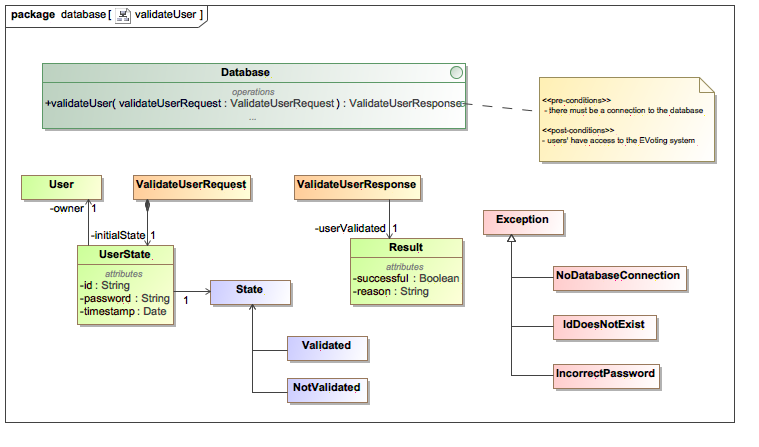
\includegraphics[width=0.75\linewidth]{../Images/Database/ServiceContracts/ValidateUser_ServiceContract.png}
					\caption{Validate User Service Contract}
				\end{figure}
				
				The system captures the ID number and password of the Voter and sends it to the Validate User functions to ensure they have been registered onto the system. After which the User will be able to access the system.
				\newline
								
				\begin{enumerate}
					\item Pre-conditions
					\begin{itemize}
						\item There must be a connection to the database
					\end{itemize}
					
					\item Exceptions
					\begin{itemize}
						\item If there is no connection to the database, the NoDatabaseConnection exception will be thrown
						\item If a user's ID is not valid, the IdDoesNotExist exception will be thrown
						\item If the user's password is entered incorrectly, the IncorrectPassword exception will be thrown
					\end{itemize}
					
					\item Post-conditions
					\begin{itemize}
						\item Users have access to the EVoting system
					\end{itemize}
				\end{enumerate}
			
			\newpage\textsl{}
			
			\item \textbf{Functional Requirements}
				\begin{figure}[H]
					\centering
					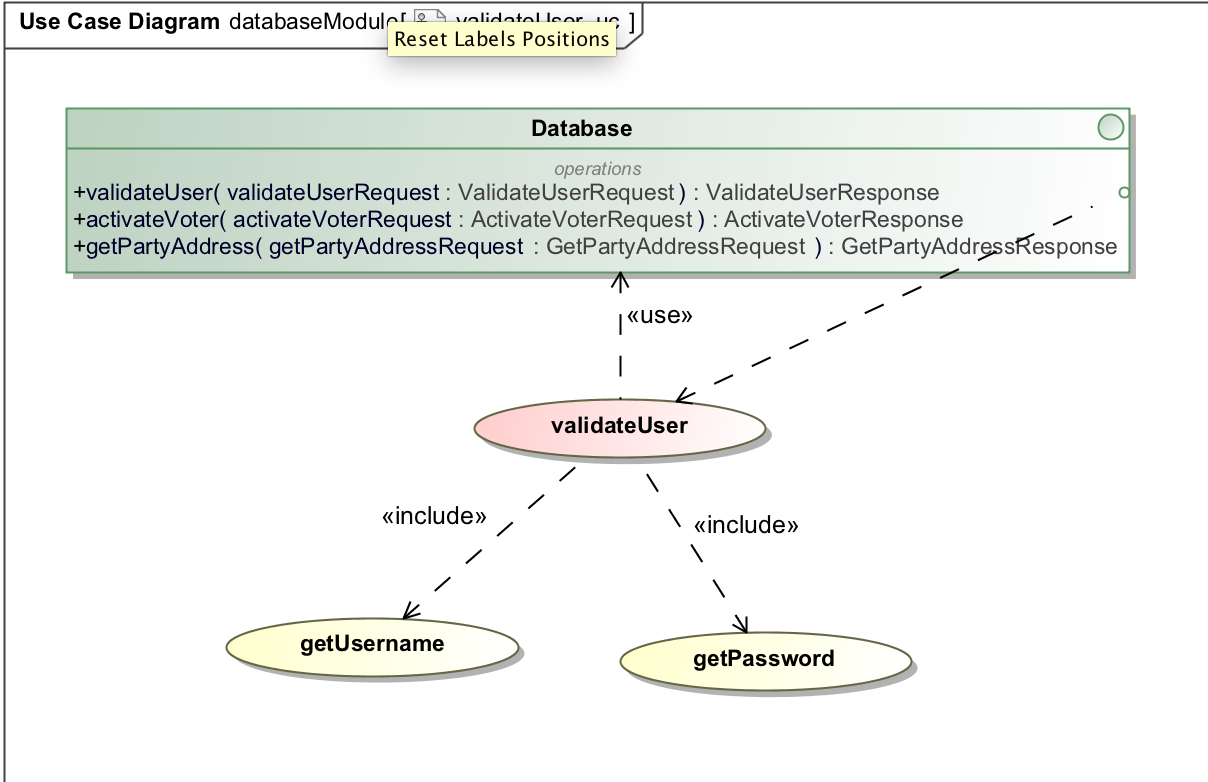
\includegraphics[width=0.75\linewidth]{../Images/Database/UseCases/ValidateUser_UseCase.png}
					\caption{Validate User Use Case}
				\end{figure}
				
			\item \textbf{Process Design}
				\begin{figure}[H]
					\centering
					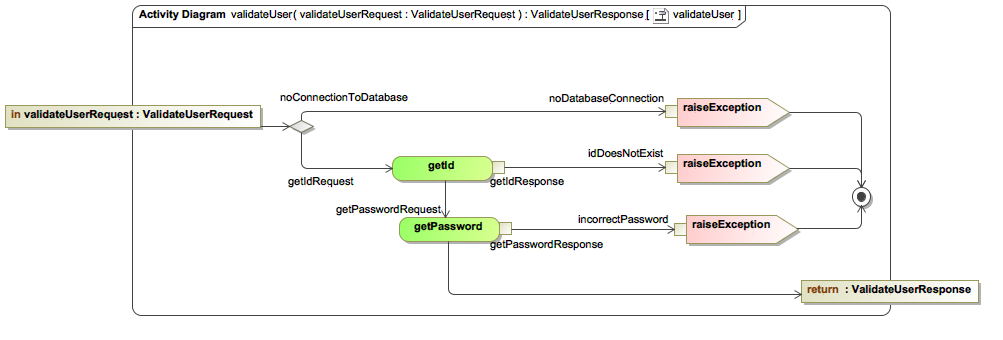
\includegraphics[width=0.75\linewidth]{../Images/Database/Activity/ValidateUser_Activity.png}
					\caption{Validate User Activity}
				\end{figure}
				
		\end{enumerate}
		
		\newpage
	
	\item \textbf{Activate User}
		\begin{enumerate}
			\item \textbf{Service Contract}
			\begin{figure}[H]
				\centering
				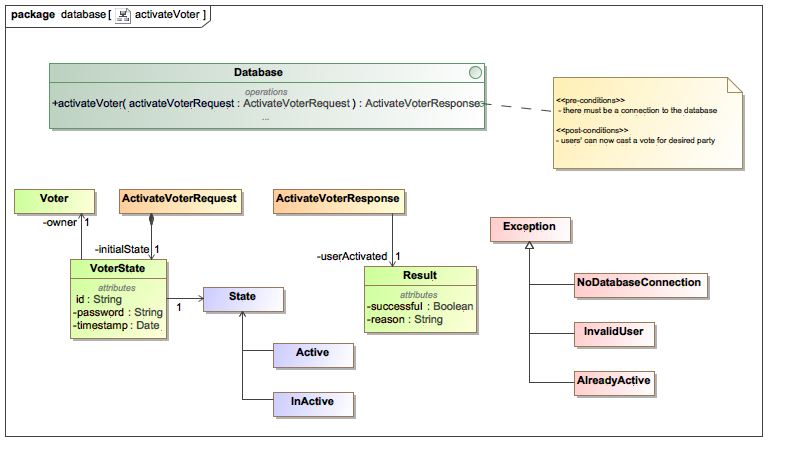
\includegraphics[width=0.75\linewidth]{../Images/Database/ServiceContracts/ActivateVoter_ServiceContract.png}
				\caption{Activate Voter Service Contract}
			\end{figure}
			
			The Activator captures the Id number of a Voter, then searches for the Voter on the system to make sure they have been registered, after which the Voter will have successfully been activated on the system.
			\newline
			
			\begin{enumerate}
				\item Pre-conditions
				\begin{itemize}
					\item There must be a connection to the database
				\end{itemize}
				
				\item Exceptions
				\begin{itemize}
						\item If there is no connection to the database, the NoDatabaseConnection exception will be thrown
						\item If a user could not be validated, the InvalidUser exception will be thrown
						\item If the user has already been activated, the AlreadyActive exception will be thrown
				\end{itemize}
				
				\item Post-conditions
				\begin{itemize}
					\item Users can now cast a vote for their desired party
				\end{itemize}
			\end{enumerate}
			
			\newpage
			
			\item \textbf{Functional Requirements}
			\begin{figure}[H]
				\centering
				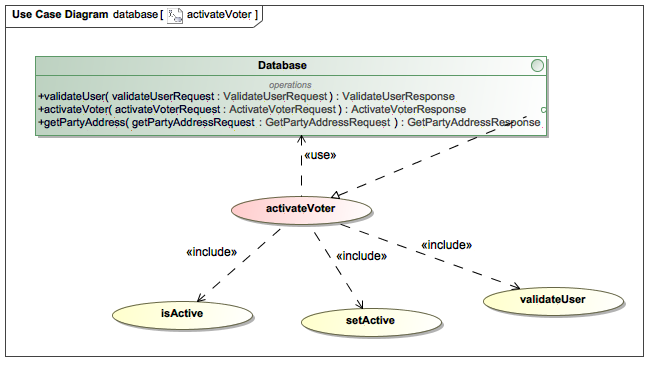
\includegraphics[width=0.75\linewidth]{../Images/Database/UseCases/ActivateVoter_UseCase.png}
				\caption{Activate Voter Use Case}
			\end{figure}
			
			\item \textbf{Process Design}
			\begin{figure}[H]
				\centering
				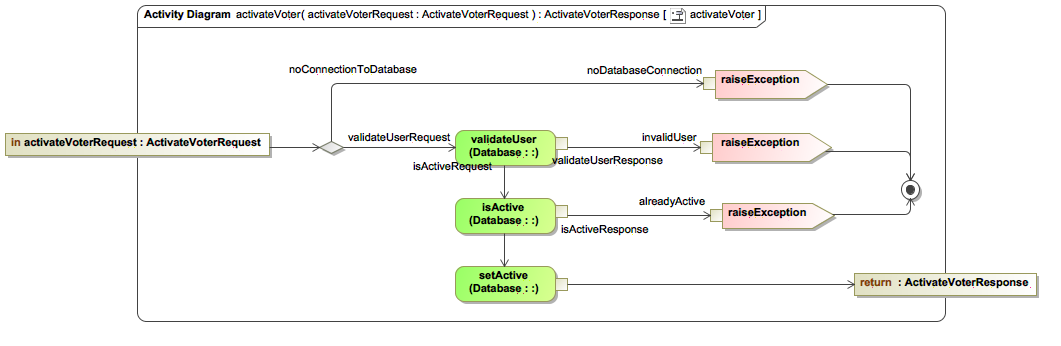
\includegraphics[width=0.75\linewidth]{../Images/Database/Activity/ActivateVoter_Activity.png}
				\caption{Activate Voter Activity}
			\end{figure}
			
		\end{enumerate}
\end{enumerate}